\chapter{Original Study: Methodology and Results}
\label{cha:original-study}

This chapter presents the completed original study as three linked experiments. \Cref{sec:shared-framework} defines the implementation, controllers, tasks, and protocol that all three experiments share. \Cref{sec:rq1} compares held-out performance, \Cref{sec:rq2} tests robustness to unseen initial weights, and \Cref{sec:rq3} examines whether lifetime updates create reusable weights.
\section{Shared Experimental Framework}
\label{sec:shared-framework}

\subsection{Implementation and Reproducibility}

Python implements the experiments, Gymnasium exposes the EvoGym environments, and PyTorch networks control the robots. A YAML configuration records the task, morphology, controller, network, evolutionary budget, evaluation protocol, runtime settings, and training seed. Before training, the implementation resolves symbolic network dimensions against the instantiated environment.

The implementation uses separate run seeds. Optimizer sampling, environment resets, and \nchl{} weight initialization therefore do not share one global generator. Before each reset, the implementation also reseeds the global Python generator for EvoGym tasks that use it internally. BidirectionalWalker, for example, selects its target direction during reset.

Each completed run stores a resolved configuration, generation-level metrics and the best genome.

\subsection{Controller Implementations}

Both conditions use the same bias-free feed-forward topology. The instantiated task and morphology determine the input width. The network contains one hidden layer with the same width as the observation vector and one output for each actuator voxel. Every layer applies a hyperbolic tangent activation:
\begin{equation}
  \mathbf{a}^{(\ell+1)}=\tanh\!\left(W^{(\ell)}\mathbf{a}^{(\ell)}\right).
  \label{eq:forward}
\end{equation}
The domain of the output is $[-1,1]$. A piecewise-linear transformation maps zero to the neutral actuator target $1.0$, negative values towards the lower action bound, and positive values towards the upper bound. This transformation preserves a meaningful neutral command when the bounds are asymmetric.

For raw network output $a_i\in[-1,1]$, lower bound $l_i$, and upper bound $u_i$, the physical actuator command is
\begin{equation}
  \widetilde{a}_i=
  \begin{cases}
    1+(1-l_i)a_i, & -1\leq a_i<0,\\
    1+(u_i-1)a_i, & 0\leq a_i\leq 1.
  \end{cases}
  \label{eq:action-mapping}
\end{equation}
Thus $a_i=-1$, $0$, and $1$ map exactly to $l_i$, $1.0$, and $u_i$, respectively.

The static condition evolves every matrix entry and loads the resulting values at the start of an episode. These weights remain fixed. The \nchl{} condition evolves per neuron parameters and samples concrete weights independently from a configured uniform interval at every episode reset. After each forward pass, the controller immediately applies the update with the pre- and postsynaptic activations cached during that pass.

The representations differ in genome length and evaluation budget, therefore the test is not a fixed compute comparison. \Cref{tab:original-settings} reports both shared and controller-specific settings.

\subsection{Tasks, Morphologies, and Evolution}

The original suite contains Walker-v0, Carrier-v0, Jumper-v0, and Thrower-v0. Every task uses the biped body; Thrower also uses a specialized arm. The two Thrower bodies differ in size and actuator count, so their comparison remains descriptive rather than controlled and is simply a study into the effect of morphology.

\begin{table}[htbp]
  \centering
  \caption{Original task--morphology conditions. The names follow the archived run configurations.}
  \label{tab:original-strata}
  \begin{tabularx}{\textwidth}{@{}llrX@{}}
    \toprule
    Task & Morphology & Horizon & Principal Behaviour \\
    \midrule
    Walker-v0 & biped & 500 & Forward locomotion on flat terrain \\
    Carrier-v0 & biped & 500 & Object transport during locomotion \\
    Jumper-v0 & biped & 500 & Vertical impulse generation \\
    Thrower-v0 & biped & 300 & Object acceleration and release \\
    Thrower-v0 & thrower\_arm & 300 & Throwing with specialized geometry \\
    \bottomrule
  \end{tabularx}
\end{table}

\begin{figure}[htbp]
  \centering
  \begin{subfigure}[t]{0.42\textwidth}
    \centering
    \setlength{\tabcolsep}{0pt}
    \begin{tabular}{cccc}
      \hactvoxel&\vactvoxel&\hactvoxel&\vactvoxel\\
      \hactvoxel&\rigidvoxel&\rigidvoxel&\vactvoxel\\
      \hactvoxel&\emptyvoxel&\emptyvoxel&\vactvoxel
    \end{tabular}
    \caption{Original-study biped.}
  \end{subfigure}
  \hfill
  \begin{subfigure}[t]{0.42\textwidth}
    \centering
    \setlength{\tabcolsep}{0pt}
    \begin{tabular}{cccccc}
      \emptyvoxel&\emptyvoxel&\rigidvoxel&\rigidvoxel&\hactvoxel&\hactvoxel\\
      \emptyvoxel&\rigidvoxel&\softvoxel&\hactvoxel&\vactvoxel&\hactvoxel\\
      \rigidvoxel&\vactvoxel&\hactvoxel&\softvoxel&\vactvoxel&\rigidvoxel\\
      \vactvoxel&\hactvoxel&\vactvoxel&\hactvoxel&\vactvoxel&\emptyvoxel\\
      \vactvoxel&\emptyvoxel&\vactvoxel&\emptyvoxel&\vactvoxel&\emptyvoxel\\
      \vactvoxel&\emptyvoxel&\vactvoxel&\emptyvoxel&\vactvoxel&\emptyvoxel
    \end{tabular}
    \caption{Specialized thrower arm.}
  \end{subfigure}

  \medskip
  \voxellegend
  \caption{Morphologies used in the original study.}
  \label{fig:original-bodies}
\end{figure}

Each combination of task, morphology, controller, and seed forms an independent optimization run. Both conditions use a population of 40 for 500 generations, select ten parents, apply Gaussian perturbation with $\sigma=0.35$, and retain the best genome observed so far. Static candidate fitness uses one episode. \nchl{} candidate fitness uses the mean of three episodes with distinct initialization and environment seed pairs in an attempt to generalize the rule across initializations.

\begin{table}[htbp]
  \centering
  \caption{Shared and controller-specific settings in the original study.}
  \label{tab:original-settings}
  \begin{tabularx}{0.94\textwidth}{@{}lX@{}}
    \toprule
    Item & Value \\
    \midrule
    Optimizer & ES1 with parent-mean Gaussian sampling and elitism \\
    Population and generations & 40 candidates and 500 generations \\
    Parent count and mutation scale & $\mu=10$ and $\sigma=0.35$ \\
    Initial evolutionary population & Uniform samples from $[-1,1]$ \\
    Candidate budget & One episode for Static-ES; three for \nchlcontroller \\
    Initial \nchl{} runtime weights & Independent uniform samples from $[-0.1,0.1]$ \\
    \nchl{} learning rate & $\eta=0.1$ \\
    Held-out evaluation & Ten episodes for each selected genome \\
    Training seeds & 0--9 \\
    \bottomrule
  \end{tabularx}
\end{table}

The evidence comprises 100 evolutionary runs, 1,000 held-out episodes, 300 weight traces, and 750 frozen-controller rollouts. The candidate evaluations add four million nested training episodes. All principal analyses use a trained run as the independent unit.

\section{RQ1: Evolutionary Training Dynamics}
\label{sec:rq1}

\subsection{Experimental Design}

This experiment uses the generation-level metrics from the ten independent evolutionary runs for each controller and task--morphology condition. At every generation, the analysis records the best fitness in the current population, the best fitness observed so far, and the population median. The curves summarize the across-run mean best-so-far fitness with a bootstrap interval and show the mean population median as a dashed line.

To determine whether the numerical fitness corresponds to recognizable task behaviour, an inspection of the footage of the best saved controller from each seed was performed. This visual assessment is qualitative: it helps distinguish genuine task completion from reward improvement that does not produce the intended behaviour.

\begin{figure}[htbp]
  \centering
  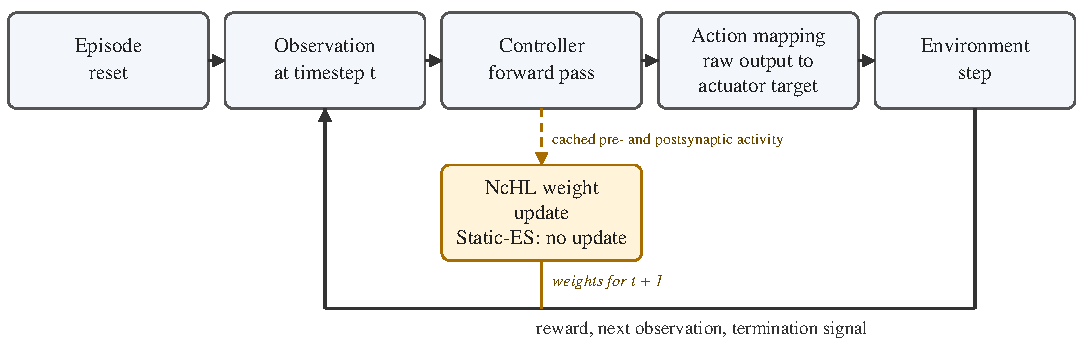
\includegraphics[width=\textwidth]{figures/training_loop.pdf}
  \caption{Within-episode control loop used to evaluate one candidate. The loop repeats until termination; accumulated reward becomes candidate fitness. The lower branch shows the additional online update performed only by \nchlcontroller.}
  \label{fig:training-loop}
\end{figure}

\subsection{Results}

The evolutionary curves show improvement for both representations. \nchlcontroller{} reaches a mean selected training fitness 4.2\% above Static-ES on Walker and 55.1\% above it on Jumper. Static-ES finishes higher on Carrier and both Thrower morphologies. \Cref{fig:evolutionary-trends} also shows substantial variation across independent runs, particularly for \nchlcontroller{}.

\begin{figure}[htbp]
  \centering
  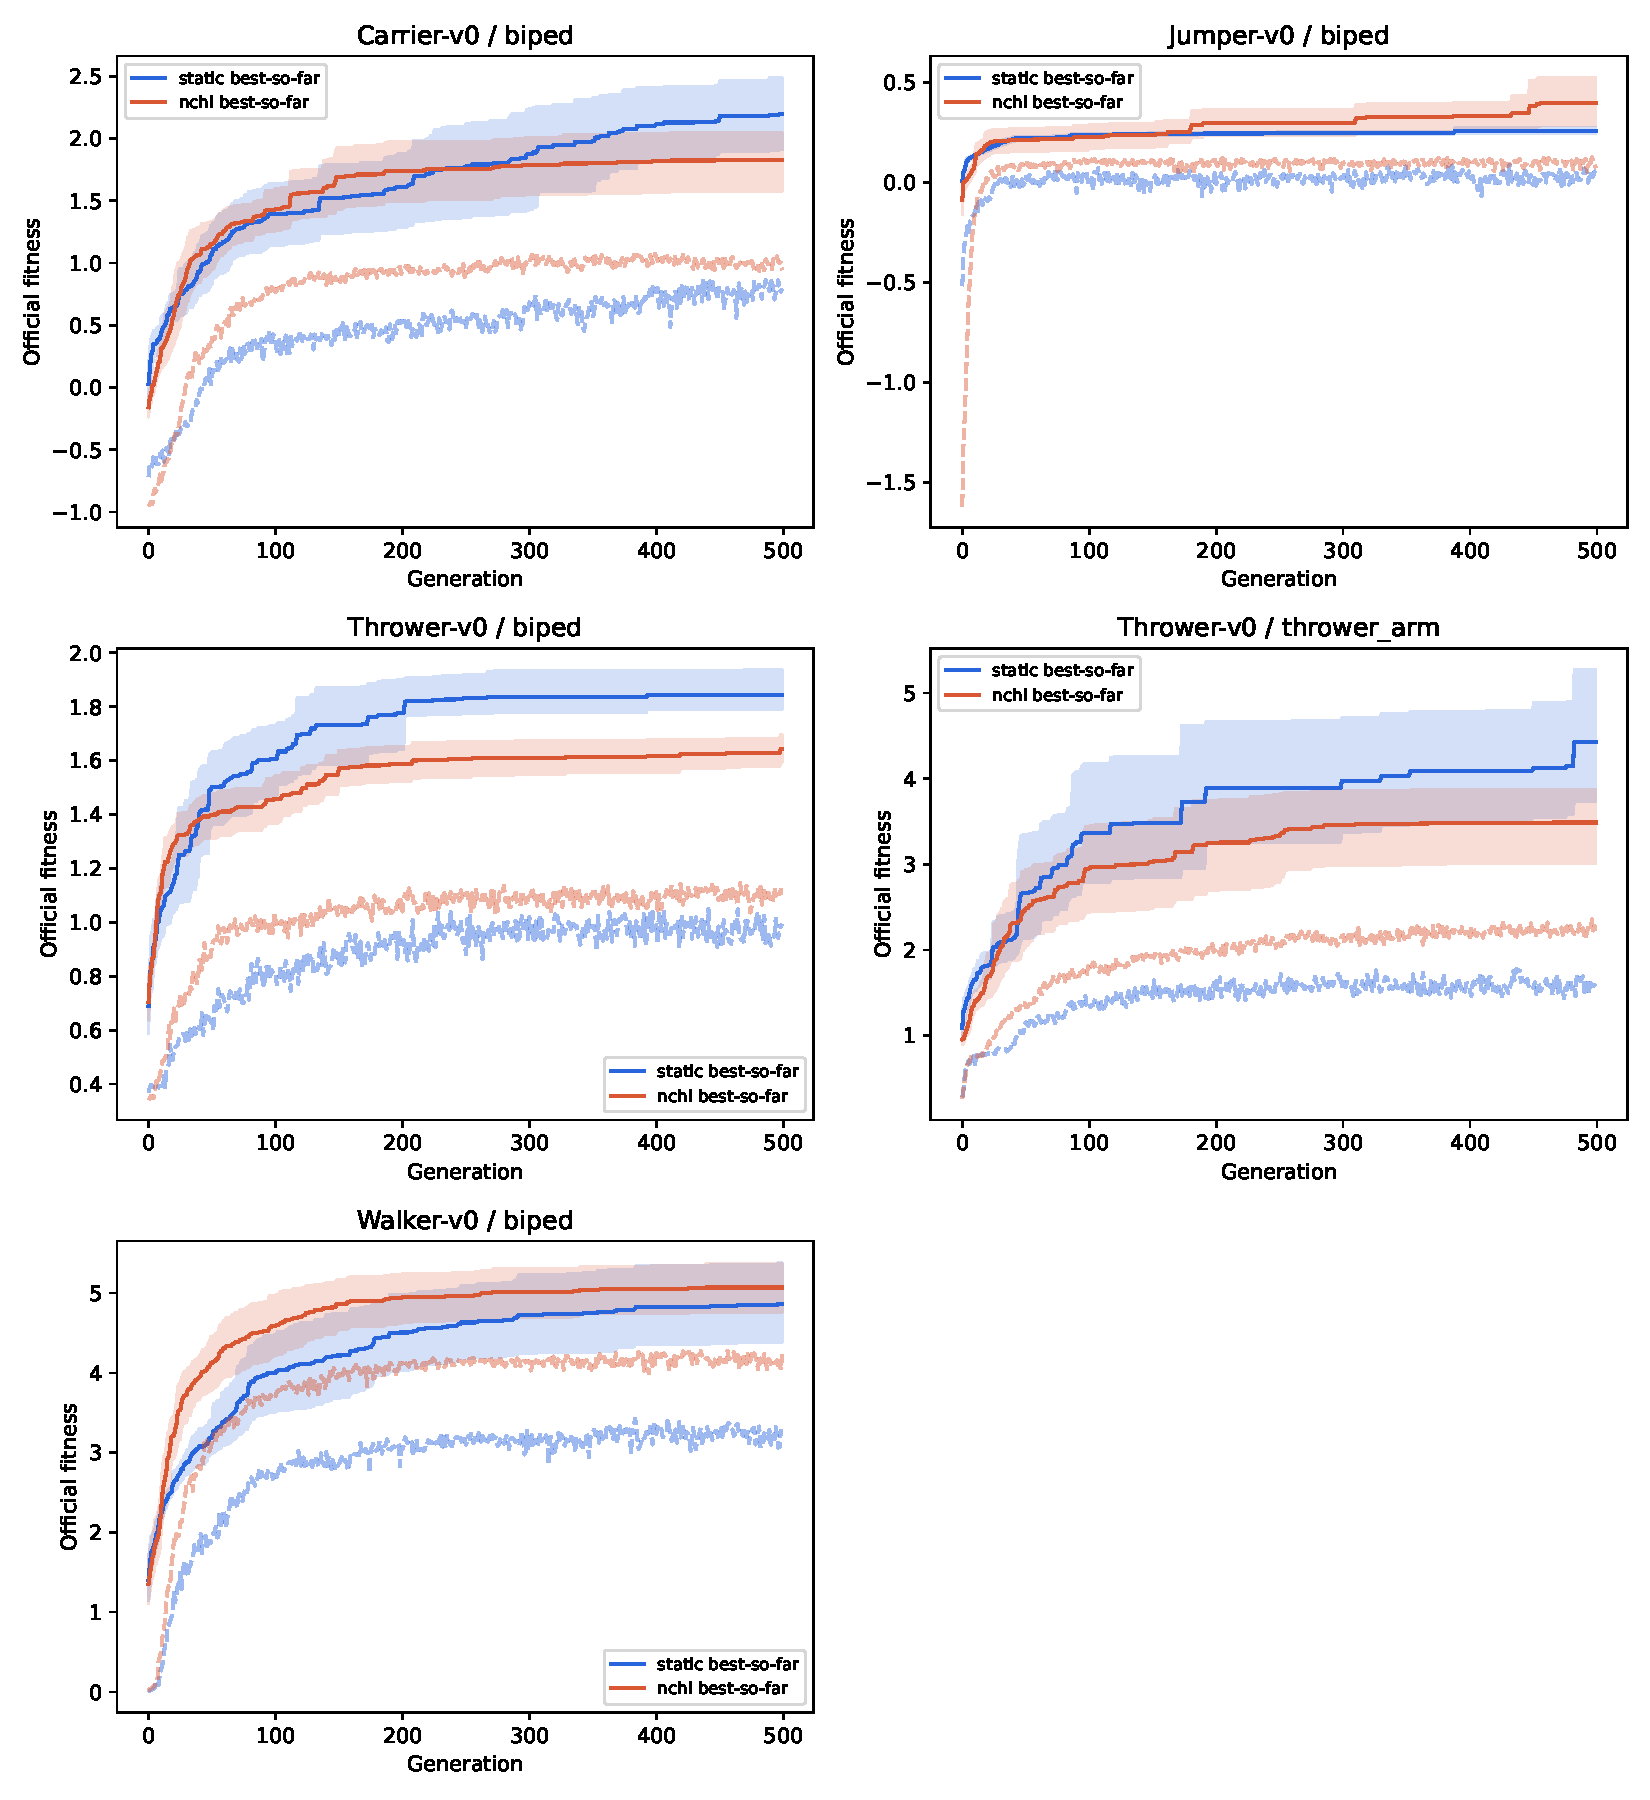
\includegraphics[width=0.98\textwidth]{figures/evolutionary_trends.pdf}
  \caption{Evolutionary training dynamics across ten runs per controller and condition. Solid lines show mean best-so-far fitness, shaded regions show bootstrap intervals, and dashed lines show the mean population median.}
  \label{fig:evolutionary-trends}
\end{figure}

The footage provides important context for these curves. On Walker, most seeds of both \nchlcontroller{} and Static-ES produce natural-looking locomotion. The biped and specialized-arm Thrower controllers can load the box and then release it with a recognizable throwing movement. These successful conditions show that \nchl{} can support both cyclical locomotion and non-cyclical, phase-structured behaviour.

Carrier and Jumper do not provide equally strong evidence. The Carrier controllers drop the box almost immediately, whereas the Jumper controllers consistently stretch upwards and then freeze; only the best examples produce a small jump. The tested morphologies and training setup therefore fail to solve these two tasks in behavioural terms. Their fitness curves still describe optimization under the task reward, but differences between \nchlcontroller{} and Static-ES in these conditions should not be treated as strong evidence about controller capability. In particular, the numerical \nchl{} advantage on Jumper does not correspond to a convincing solution of the task.

\paragraph{RQ1 Summary.} Both representations improve during evolution, but the fitness curves do not always indicate successful task behaviour. Walker and both Thrower morphologies produce meaningful solutions, demonstrating that \nchl{} can support both cyclical and phase-structured control. Carrier and Jumper remain behaviourally unsolved with the tested morphologies, so their relative fitness values provide weak evidence for comparing the controllers.

\clearpage
\section{RQ2: Robustness to Unseen Initial Weights}
\label{sec:rq2}

\subsection{Experimental Design}

An \nchl{} genome encodes a rule rather than one final weight matrix. This experiment applies every selected rule to initial weights generated from seeds outside its training stream. The ten held-out episodes for each run vary both the environment seed and controller seed. Because the original nominal environments behave deterministically after their declared reset, the sampled runtime weights dominate the additional within-run dispersion.

We compare the selected training fitness for each run---the maximum three-episode candidate estimate observed during evolution---with the mean over ten held-out initializations. The difference addresses practical generalization but can combine three mechanisms: specialization to fixed training pairs, optimism from selecting the maximum noisy estimate, and an inability to recover from arbitrary $W_0$. This design establishes the gap but cannot separate those causes.

\subsection{Results}

All 50 selected \nchl{} solutions achieve a lower mean across ten unseen initial weights than their selected three-initialization training estimate. \Cref{tab:rq2-generalization} reports the condition means. Retained performance divides the held-out mean by the selected training mean.

\begin{table}[htbp]
  \centering
  \small
  \caption{Generalization of selected \nchl{} rules to unseen runtime-weight initializations. Within-run SD summarizes ten nested episodes.}
  \label{tab:rq2-generalization}
  \begin{tabular}{@{}lrrrrrr@{}}
    \toprule
    Condition & Training & Held-out & Gap & Retained & Within-run SD & Negative Episodes \\
    \midrule
    Walker, biped & 5.069 & 4.395 & $-0.674$ & 86.7\% & 0.691 & 1/100 \\
    Carrier, biped & 1.825 & 1.191 & $-0.634$ & 65.3\% & 0.464 & 3/100 \\
    Jumper, biped & 0.399 & 0.024 & $-0.375$ & 6.0\% & 0.369 & 35/100 \\
    Thrower, biped & 1.643 & 1.215 & $-0.429$ & 73.9\% & 0.289 & 2/100 \\
    Thrower, arm & 3.488 & 2.233 & $-1.255$ & 64.0\% & 0.613 & 8/100 \\
    \bottomrule
  \end{tabular}
\end{table}

Jumper provides the strongest failure case. Its held-out mean retains only 6.0\% of the selected training mean, four of ten run means become negative, and 35 of 100 nested episodes produce negative return. Walker retains 86.7\%, whereas Carrier and the two Thrower conditions retain approximately 64--74\%. Static-ES reproduces its selected weights during evaluation and therefore has no corresponding variation from weight initialization.

Evolution evaluates three fixed initialization pairs per run and selects the best noisy candidate encountered across 500 generations. Lower held-out performance can therefore reflect specialization, selection optimism, or insufficient recovery from arbitrary starting weights. The data establish the practical result that new runtime weights remain consequential in every condition.

\paragraph{RQ2 Summary.} The results indicate that weight initialization influences the behaviour produced by the evolved learning rules. Nevertheless, the Walker and Thrower controllers retain meaningful task behaviour across initializations, suggesting that the rules capture useful structure rather than relying on a single favourable initialization. The poor performance on Carrier and Jumper is less informative about robustness because these tasks were not successfully learned under the nominal evaluation either.

\section{RQ3: Do Lifetime Updates Create Useful Weights?}
\label{sec:rq3}

\subsection{Freeze-and-Replay Design}

This experiment reuses the best \nchl{} genome from every original run and performs no further evolutionary search. Three independently seeded plastic source episodes generate concrete weight matrices at five normalized lifetime positions:
\begin{equation}
  W_0,\quad W_{25},\quad W_{50},\quad W_{75},\quad W_{\mathrm{final}}.
\end{equation}
The trace records $W_0$ before the first action. It records $W_{\mathrm{final}}$ after the update that follows the last source action, so this final matrix might never generate an action in the source trajectory.

The replay procedure loads each matrix into a static network and starts a fresh episode with the environment seed of the corresponding source trace. It disables plasticity throughout replay. This intervention tests whether an acquired matrix remains useful from the normal initial state; it does not continue from the physical state that produced the matrix.

For every snapshot, we first average the three traces within each evolutionary run and then summarize the runs. The principal quantities are the frozen-fitness change from $W_0$, the lifetime stage with the best frozen fitness, and the difference between the fully plastic source return and each frozen controller. Improvement over $W_0$ supports lifetime improvement.

\subsection{Results}

The experiment starts from a deliberately weak baseline. Before adaptation, random $W_0$ networks produce near-zero Walker fitness, negative Carrier and Jumper fitness, and low Thrower fitness. Later snapshots acquire useful fresh-start behaviour in several conditions, but the pattern is neither uniform nor monotonic (\Cref{tab:rq3-freeze}).

\begin{table}[htbp]
  \centering
  \scriptsize
  \caption{Fresh-start frozen fitness across lifetime snapshots. Values first average three traces within each run and then average ten run means. ``Improved'' counts runs for which $W_{\mathrm{final}}$ exceeds $W_0$.}
  \label{tab:rq3-freeze}
  \begin{tabular}{@{}lrrrrrrrr@{}}
    \toprule
    Condition & Plastic & $W_0$ & $W_{25}$ & $W_{50}$ & $W_{75}$ & $W_{final}$ & Final Change & Improved \\
    \midrule
    Walker, biped & 4.557 & 0.000 & 2.263 & 2.242 & 2.030 & 2.381 & $+2.381$ & 8/10 \\
    Carrier, biped & 1.276 & $-0.490$ & $-0.083$ & $-0.019$ & $-0.017$ & 0.004 & $+0.493$ & 7/10 \\
    Jumper, biped & 0.167 & $-0.168$ & $-2.133$ & $-2.912$ & $-2.705$ & $-2.093$ & $-1.925$ & 0/10 \\
    Thrower, biped & 1.248 & 0.338 & 0.338 & 0.346 & 0.482 & 0.498 & $+0.160$ & 8/10 \\
    Thrower, arm & 2.252 & 0.243 & 1.087 & 1.037 & 1.172 & 1.369 & $+1.125$ & 9/10 \\
    \bottomrule
  \end{tabular}
\end{table}

\begin{figure}[htbp]
  \centering
  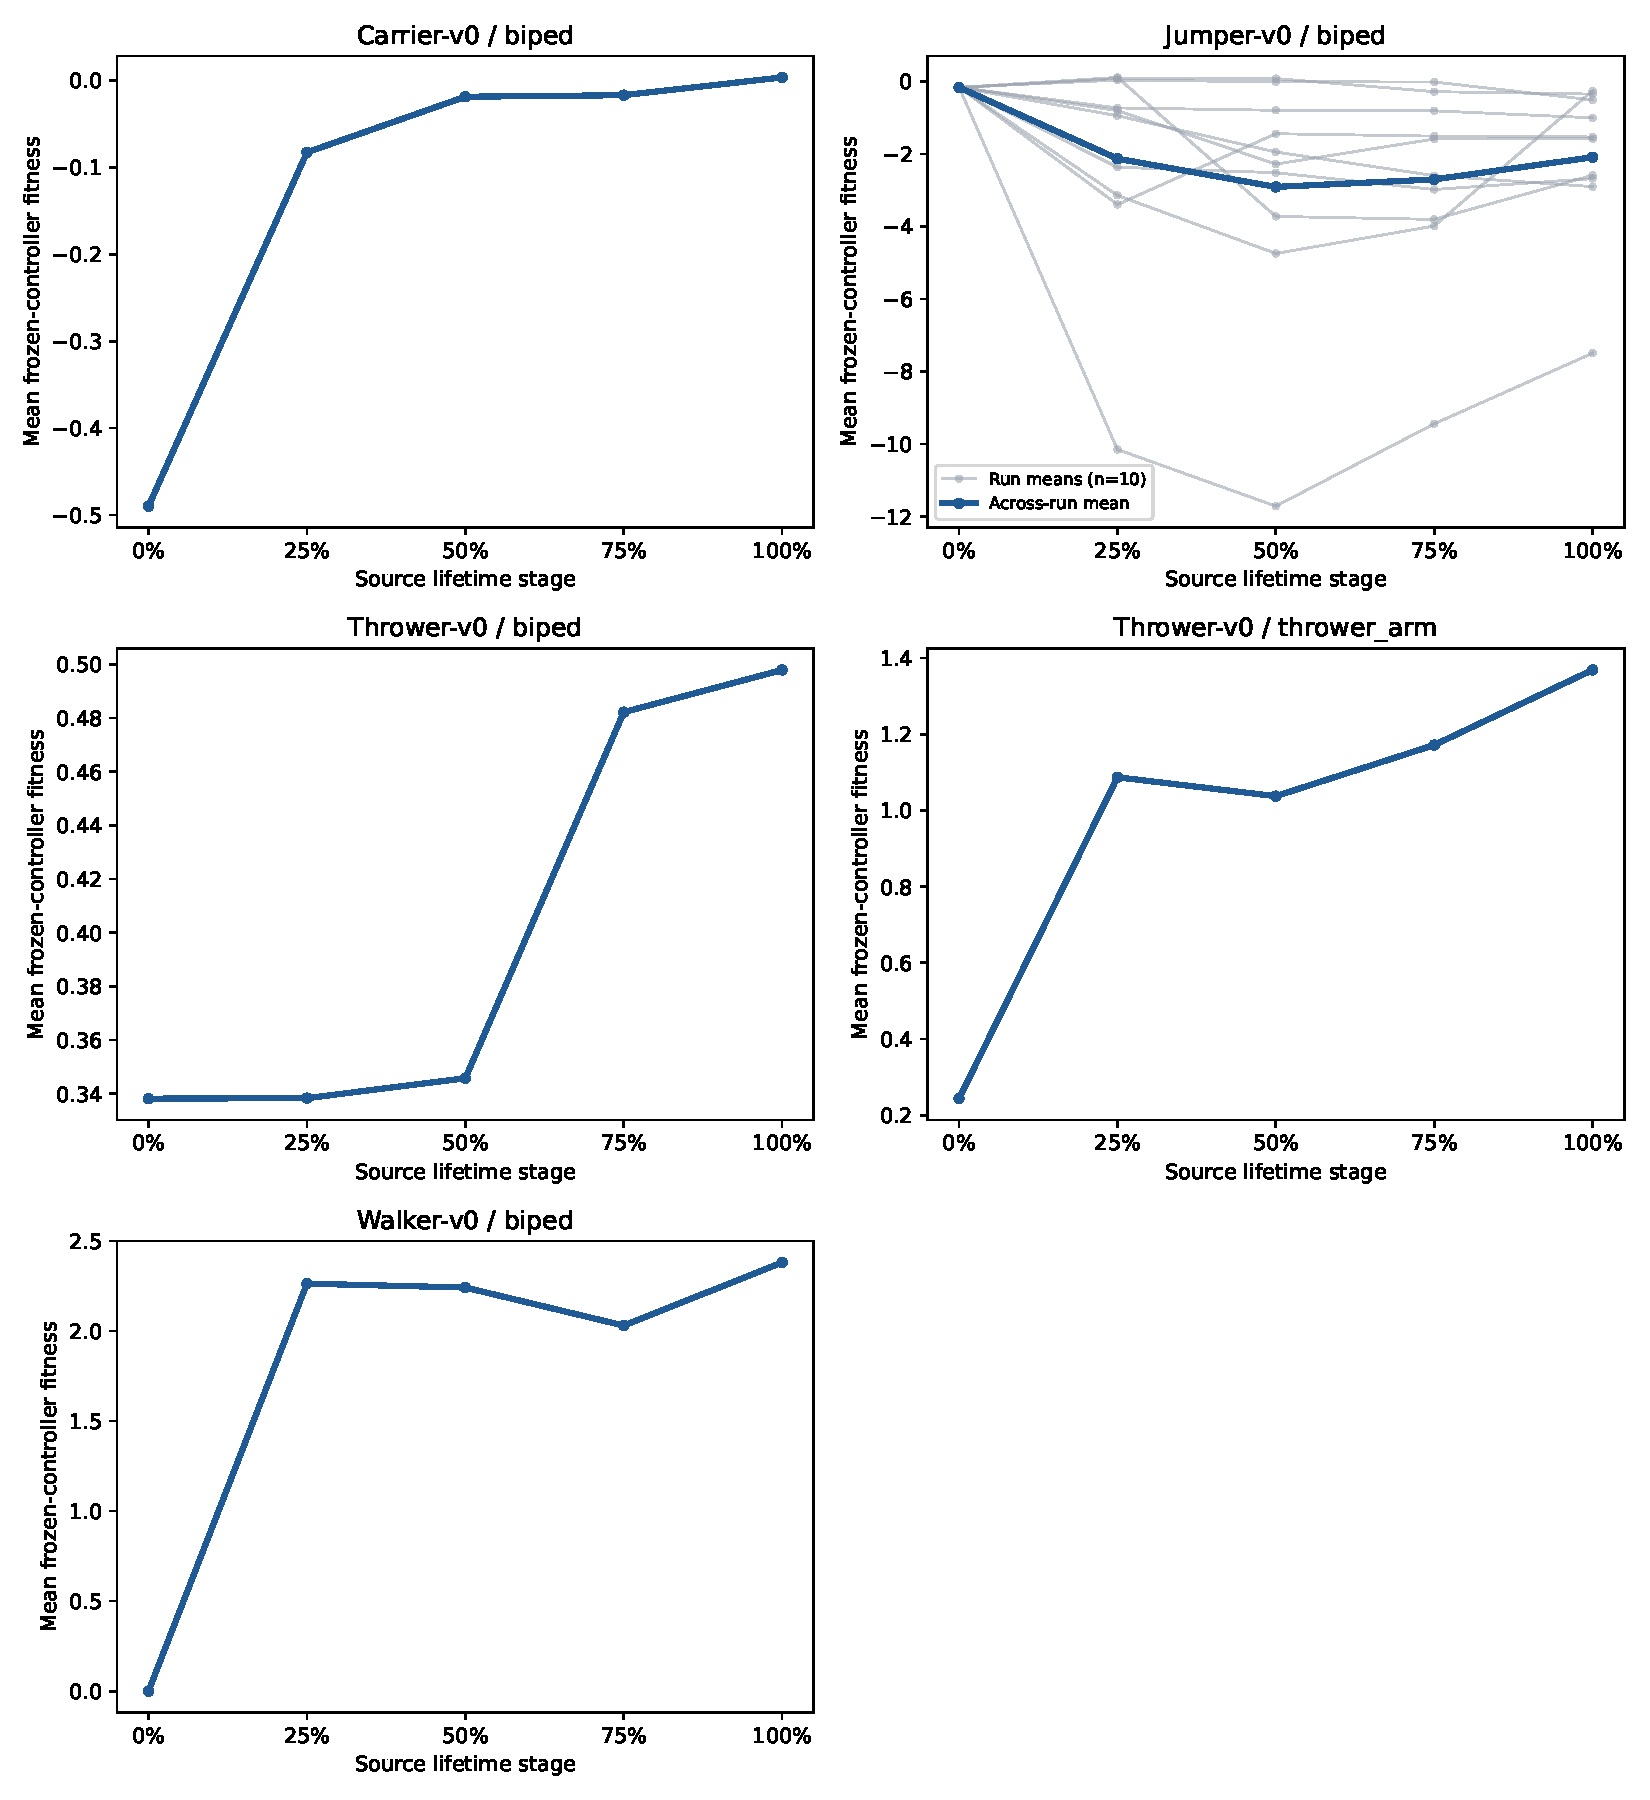
\includegraphics[width=0.98\textwidth]{figures/freeze_fitness_over_lifetime.pdf}
  \caption{Across-run mean fitness of frozen weight snapshots evaluated from a fresh task start. The Jumper panel retains the ten run means in grey to illustrate the large between-seed variation; the blue line gives the across-run mean in every panel.}
  \label{fig:freeze-fitness}
\end{figure}

Plastic control outperforms the matched $W_0$ frozen ablation in 49 of 50 runs. It also exceeds $W_{\mathrm{final}}$ in 47 runs and the post-hoc best frozen snapshot in 46. 

Only five of the 50 frozen trajectories improve monotonically across all five snapshots. The learning rule therefore does not simply approach one final static optimum. A late matrix can perform poorly from the initial physical state while remaining useful during the phase that produced it.

\paragraph{RQ3 Summary.} Online updates contribute to performance, but they do not generally converge towards one progressively better fixed controller. The Walker result however is interesting: its highest frozen fitness occurs at \(W_{\mathrm{final}}\), suggesting that tasks with periodic optimal movement may show an upward fitness trend as the repeated control loop is progressively optimized.

